\documentclass[11pt]{article}
\usepackage[margin=0.95in]{geometry}
\usepackage{lmodern}
\usepackage[T1]{fontenc}
\usepackage{microtype}
\usepackage{xcolor}
\usepackage{amsmath,amssymb,mathtools}
\usepackage{booktabs,tabularx,longtable,array,multirow}
\newcolumntype{Y}{>{\raggedright\arraybackslash}X}
\usepackage{enumitem}
\usepackage{caption}
\usepackage{listings}
\usepackage{tikz}
\usetikzlibrary{arrows.meta,positioning,shapes.geometric,calc}
\usepackage[hidelinks]{hyperref}

\definecolor{navy}{HTML}{1B3A4B}
\definecolor{teal}{HTML}{0E6B66}
\definecolor{tealfaint}{HTML}{E5F3F1}
\definecolor{gold}{HTML}{A56B10}
\definecolor{goldfaint}{HTML}{FBF3E0}
\definecolor{brick}{HTML}{8E3A3A}
\definecolor{brickfaint}{HTML}{F8E8E6}
\definecolor{leaf}{HTML}{2F6F4E}
\definecolor{leaffaint}{HTML}{E5F2EA}
\definecolor{slate}{HTML}{5E6A75}
\definecolor{linec}{HTML}{243140}
\definecolor{paper}{HTML}{F7F4EF}
\definecolor{unk}{HTML}{E4E1DA}
\definecolor{freec}{HTML}{F7F7F5}
\definecolor{occ}{HTML}{2C333A}
\definecolor{enc}{HTML}{C45C4A}
\definecolor{frcell}{HTML}{2A9D8F}
\definecolor{codebg}{HTML}{F4F1EA}

\lstset{
  basicstyle=\ttfamily\footnotesize,
  backgroundcolor=\color{codebg},
  frame=single,
  rulecolor=\color{linec},
  breaklines=true,
  columns=fullflexible,
  keepspaces=true,
  xleftmargin=1em,
  framexleftmargin=0.6em
}

\setlist[itemize]{leftmargin=1.2em, itemsep=0.2em, topsep=0.35em}
\setlist[enumerate]{leftmargin=1.4em, itemsep=0.25em, topsep=0.35em}
\captionsetup{font=small, labelfont=bf, skip=6pt}
\setlength{\parskip}{0.35em}
\setlength{\parindent}{1.15em}
\setlength{\emergencystretch}{2em}
\renewcommand{\arraystretch}{1.15}

\newcommand{\code}[1]{\texttt{#1}}
\newcommand{\commit}[1]{\texttt{#1}}

% Shared technical figures. Each command emits a tikzpicture only.
% Captions and labels live in the manuscripts so the two papers can differ.

\newcommand{\FigArchitecture}{%
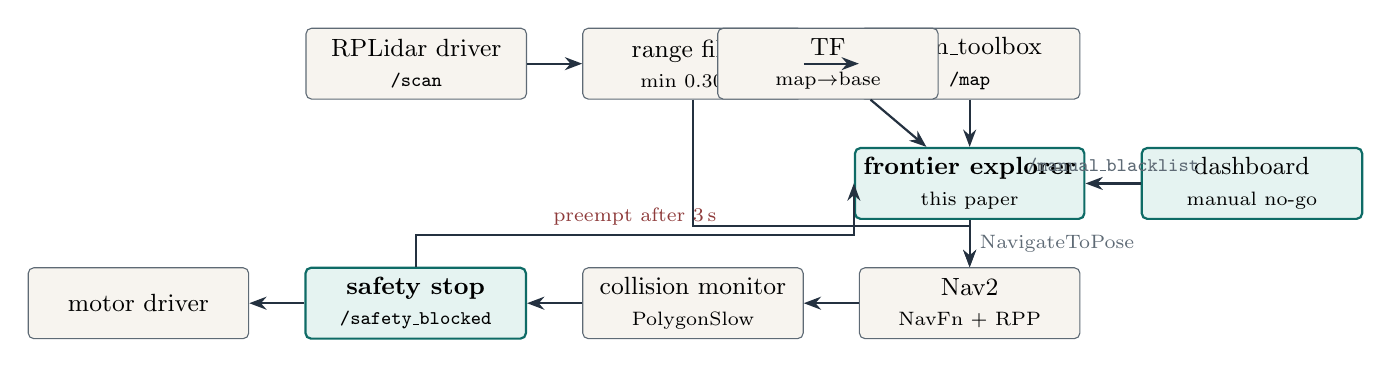
\begin{tikzpicture}[
  font=\small,
  node distance=6mm and 7mm,
  box/.style={draw=linec, rounded corners=2pt, align=center, fill=white,
              minimum width=28mm, minimum height=9mm, inner sep=3pt},
  custom/.style={box, fill=tealfaint, draw=teal, thick},
  oss/.style={box, fill=paper, draw=slate},
  arr/.style={-{Stealth[length=2.2mm]}, draw=linec, thick}
]
  \node[oss] (lidar) {RPLidar driver\\{\scriptsize\texttt{/scan}}};
  \node[oss, right=of lidar] (filter) {range filter\\{\scriptsize min 0.30\,m}};
  \node[oss, right=of filter] (slam) {slam\_toolbox\\{\scriptsize\texttt{/map}}};
  \node[custom, below=of slam] (expl) {\textbf{frontier explorer}\\{\scriptsize this paper}};
  \node[oss, below=of expl] (nav) {Nav2\\{\scriptsize NavFn + RPP}};
  \node[oss, left=of nav] (coll) {collision monitor\\{\scriptsize PolygonSlow}};
  \node[custom, left=of coll] (safe) {\textbf{safety stop}\\{\scriptsize\texttt{/safety\_blocked}}};
  \node[oss, left=of safe] (drv) {motor driver};
  \node[oss, above=of expl, xshift=-18mm] (tf) {TF\\{\scriptsize map$\rightarrow$base}};
  \node[custom, right=of expl] (dash) {dashboard\\{\scriptsize manual no-go}};

  \draw[arr] (lidar) -- (filter);
  \draw[arr] (filter) -- (slam);
  \draw[arr] (slam) -- (expl);
  \draw[arr] (expl) -- node[right, font=\scriptsize, text=slate] {NavigateToPose} (nav);
  \draw[arr] (nav) -- (coll);
  \draw[arr] (coll) -- (safe);
  \draw[arr] (safe) -- (drv);
  \draw[arr] (tf) -- (expl);
  \draw[arr] (dash) -- node[above, font=\scriptsize, text=slate] {\texttt{/manual\_blacklist}} (expl);
  \draw[arr] (safe.north) -- ++(0,4mm) -| node[pos=0.25, above, font=\scriptsize, text=brick] {preempt after 3\,s} (expl.west);
  \draw[arr] (filter.south) -- ++(0,-16mm) -| (nav.north);
\end{tikzpicture}%
}

\newcommand{\FigCommandChain}{%
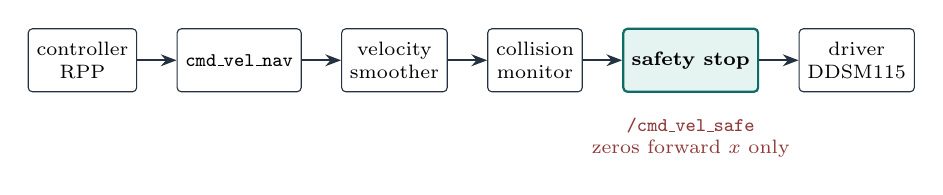
\begin{tikzpicture}[
  font=\scriptsize,
  arr/.style={-{Stealth[length=2mm]}, draw=linec, thick},
  n/.style={draw=linec, rounded corners=1.5pt, align=center, fill=white,
            inner sep=3pt, minimum height=8mm},
  c/.style={n, fill=tealfaint, draw=teal, thick}
]
  \node[n] (a) {controller\\RPP};
  \node[n, right=5mm of a] (b) {\texttt{cmd\_vel\_nav}};
  \node[n, right=5mm of b] (c) {velocity\\smoother};
  \node[n, right=5mm of c] (d) {collision\\monitor};
  \node[c, right=5mm of d] (e) {\textbf{safety stop}};
  \node[n, right=5mm of e] (f) {driver\\DDSM115};
  \draw[arr] (a) -- (b);
  \draw[arr] (b) -- (c);
  \draw[arr] (c) -- (d);
  \draw[arr] (d) -- (e);
  \draw[arr] (e) -- (f);
  \node[below=2mm of e, align=center, text=brick, font=\scriptsize]
    {\texttt{/cmd\_vel\_safe}\\zeros forward $x$ only};
\end{tikzpicture}%
}

\newcommand{\FigPipeline}{%
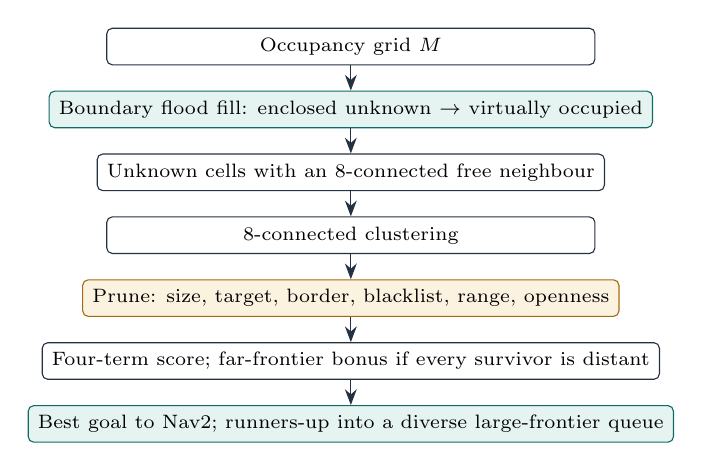
\begin{tikzpicture}[
  font=\scriptsize,
  node distance=3.2mm,
  s/.style={draw=linec, rounded corners=2pt, align=center, fill=white,
            minimum width=62mm, inner sep=3.5pt},
  d/.style={s, fill=goldfaint, draw=gold},
  k/.style={s, fill=tealfaint, draw=teal},
  arr/.style={-{Stealth[length=2mm]}, draw=linec}
]
  \node[s] (m) {Occupancy grid $M$};
  \node[k, below=of m] (e) {Boundary flood fill: enclosed unknown $\rightarrow$ virtually occupied};
  \node[s, below=of e] (f) {Unknown cells with an 8-connected free neighbour};
  \node[s, below=of f] (c) {8-connected clustering};
  \node[d, below=of c] (p) {Prune: size, target, border, blacklist, range, openness};
  \node[s, below=of p] (sc) {Four-term score; far-frontier bonus if every survivor is distant};
  \node[k, below=of sc] (q) {Best goal to Nav2; runners-up into a diverse large-frontier queue};
  \draw[arr] (m) -- (e);
  \draw[arr] (e) -- (f);
  \draw[arr] (f) -- (c);
  \draw[arr] (c) -- (p);
  \draw[arr] (p) -- (sc);
  \draw[arr] (sc) -- (q);
\end{tikzpicture}%
}

\newcommand{\FigEnclosed}{%
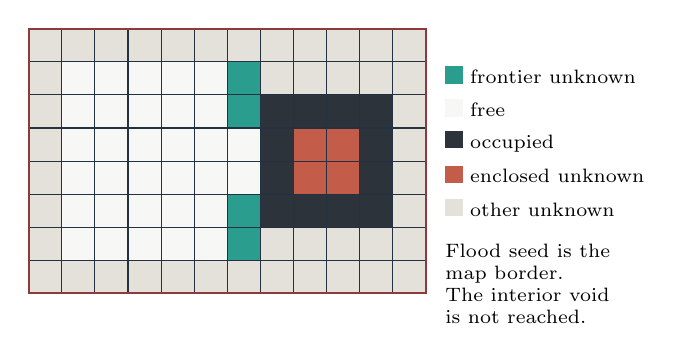
\begin{tikzpicture}[scale=0.42, font=\scriptsize]
  \foreach \x in {0,...,11} {
    \foreach \y in {0,...,7} {
      \fill[unk] (\x,\y) rectangle ++(1,1);
    }
  }
  % reachable free corridor and room
  \foreach \x/\y in {1/1,2/1,3/1,4/1,5/1,1/2,2/2,3/2,4/2,5/2,1/3,2/3,3/3,4/3,5/3,6/3,1/4,2/4,3/4,4/4,5/4,6/4,1/5,2/5,3/5,4/5,5/5,1/6,2/6,3/6,4/6,5/6} {
    \fill[freec] (\x,\y) rectangle ++(1,1);
  }
  % obstacle shell
  \foreach \x/\y in {7/2,8/2,9/2,10/2,7/3,10/3,7/4,10/4,7/5,8/5,9/5,10/5} {
    \fill[occ] (\x,\y) rectangle ++(1,1);
  }
  % enclosed unknown inside the shell
  \foreach \x/\y in {8/3,9/3,8/4,9/4} {
    \fill[enc] (\x,\y) rectangle ++(1,1);
  }
  % frontier-like unknown touching free on the right of the room
  \foreach \x/\y in {6/1,6/2,6/5,6/6} {
    \fill[frcell] (\x,\y) rectangle ++(1,1);
  }
  \draw[linec, thin] (0,0) grid (12,8);
  \draw[brick, thick] (0,0) rectangle (12,8);
  \node[anchor=west, font=\scriptsize] at (12.3,6.6) {\textcolor{frcell}{\rule{2.2mm}{2.2mm}} frontier unknown};
  \node[anchor=west, font=\scriptsize] at (12.3,5.6) {\textcolor{freec}{\rule{2.2mm}{2.2mm}} free};
  \node[anchor=west, font=\scriptsize] at (12.3,4.6) {\textcolor{occ}{\rule{2.2mm}{2.2mm}} occupied};
  \node[anchor=west, font=\scriptsize] at (12.3,3.6) {\textcolor{enc}{\rule{2.2mm}{2.2mm}} enclosed unknown};
  \node[anchor=west, font=\scriptsize] at (12.3,2.6) {\textcolor{unk}{\rule{2.2mm}{2.2mm}} other unknown};
  \node[align=left, anchor=north west, font=\scriptsize] at (12.3,1.8)
    {Flood seed is the\\map border.\\The interior void\\is not reached.};
\end{tikzpicture}%
}

\newcommand{\FigPrune}{%
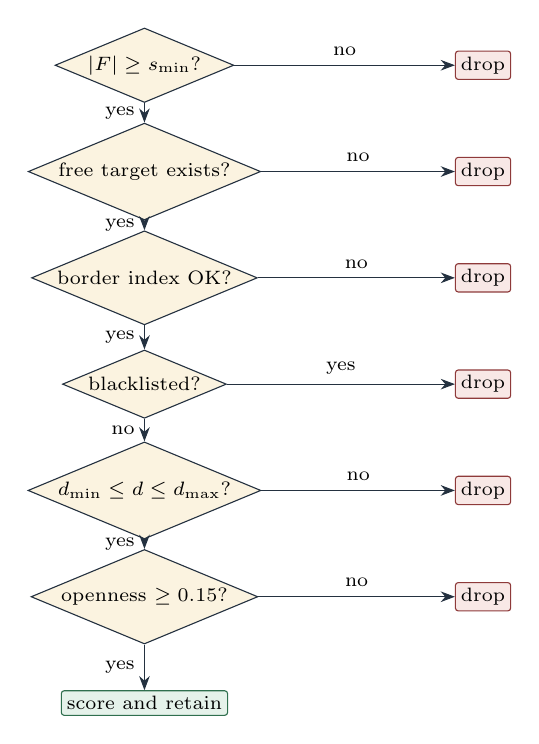
\begin{tikzpicture}[
  font=\scriptsize,
  dec/.style={draw=linec, diamond, aspect=2.4, align=center, inner sep=1pt, fill=goldfaint},
  rej/.style={draw=brick, fill=brickfaint, rounded corners=1pt, align=center, inner sep=2pt},
  ok/.style={draw=leaf, fill=leaffaint, rounded corners=1pt, align=center, inner sep=2pt},
  arr/.style={-{Stealth[length=1.8mm]}, draw=linec}
]
  \node[dec] (s) at (0,0) {$|F|\ge s_{\min}$?};
  \node[rej] (r1) at (4.3,0) {drop};
  \node[dec] (t) at (0,-1.35) {free target exists?};
  \node[rej] (r2) at (4.3,-1.35) {drop};
  \node[dec] (b) at (0,-2.7) {border index OK?};
  \node[rej] (r3) at (4.3,-2.7) {drop};
  \node[dec] (k) at (0,-4.05) {blacklisted?};
  \node[rej] (r4) at (4.3,-4.05) {drop};
  \node[dec] (d) at (0,-5.4) {$d_{\min}\le d\le d_{\max}$?};
  \node[rej] (r5) at (4.3,-5.4) {drop};
  \node[dec] (o) at (0,-6.75) {openness $\ge 0.15$?};
  \node[rej] (r6) at (4.3,-6.75) {drop};
  \node[ok] (g) at (0,-8.1) {score and retain};
  \draw[arr] (s) -- node[left] {yes} (t);
  \draw[arr] (s) -- node[above] {no} (r1);
  \draw[arr] (t) -- node[left] {yes} (b);
  \draw[arr] (t) -- node[above] {no} (r2);
  \draw[arr] (b) -- node[left] {yes} (k);
  \draw[arr] (b) -- node[above] {no} (r3);
  \draw[arr] (k) -- node[left] {no} (d);
  \draw[arr] (k) -- node[above] {yes} (r4);
  \draw[arr] (d) -- node[left] {yes} (o);
  \draw[arr] (d) -- node[above] {no} (r5);
  \draw[arr] (o) -- node[left] {yes} (g);
  \draw[arr] (o) -- node[above] {no} (r6);
\end{tikzpicture}%
}

\newcommand{\FigScore}{%
\begin{tikzpicture}[x=1.15cm, y=0.55cm, font=\scriptsize]
  \draw[linec] (0,0) -- (0,5.2);
  \draw[linec] (0,2.6) -- (8.6,2.6);
  \node[rotate=90, anchor=south] at (-0.45,2.6) {contribution};
  % zero line at y=2.6; scale 4 units per 1.0 score
  \foreach \y/\lab in {0.6/-0.5, 2.6/0, 4.6/+0.5} {
    \draw[slate] (-0.08,\y) -- (0.08,\y);
  }
  \node[left] at (0,0.6) {$-0.5$};
  \node[left] at (0,2.6) {$0$};
  \node[left] at (0,4.6) {$+0.5$};
  % A contributions: +0.90, -0.40, -0.25, +0.42  but bars relative to zero
  % clip display: size +0.90 is off scale if 4 per unit... use 2.2 per unit
  % redo: unit = 2.2 cm per 1.0, zero at 0
  % I'll draw from scratch with y unit already set. Let me use absolute.
\end{tikzpicture}%
}

% The placeholder above is replaced by a real waterfall. Defined separately.
\renewcommand{\FigScore}{%
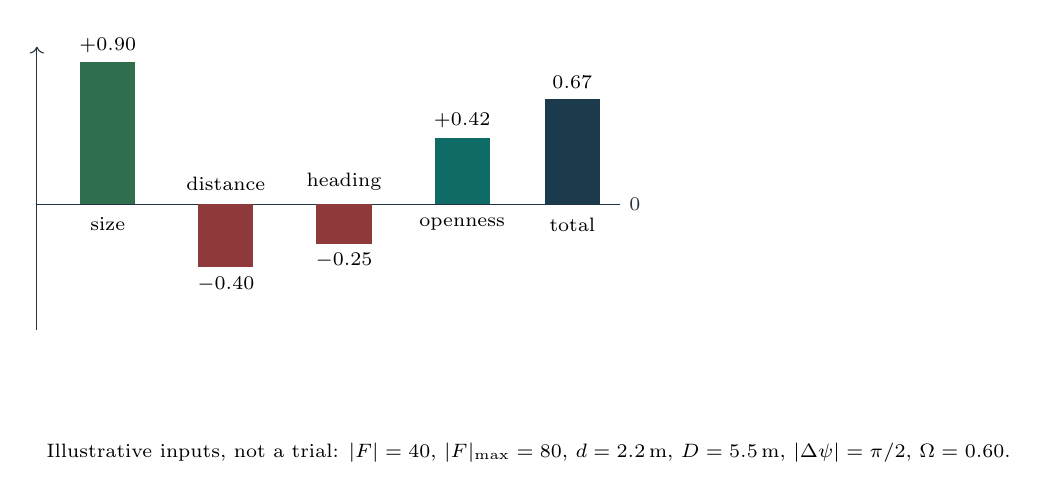
\begin{tikzpicture}[font=\scriptsize]
  \def\z{0}
  % bars: size +0.90, dist -0.40, head -0.25, open +0.42, total 0.67
  \draw[->, linec] (0,0) -- (0,3.6) node[above] {};
  \draw[linec] (0,1.6) -- (7.4,1.6) node[right] {$0$};
  \begin{scope}[shift={(0.55,1.6)}]
    \fill[leaf] (0,0) rectangle (0.7,1.80);
    \node[above] at (0.35,1.80) {$+0.90$};
    \node[below] at (0.35,-0.05) {size};
  \end{scope}
  \begin{scope}[shift={(2.05,1.6)}]
    \fill[brick] (0,-0.80) rectangle (0.7,0);
    \node[below] at (0.35,-0.80) {$-0.40$};
    \node[above] at (0.35,0.05) {distance};
  \end{scope}
  \begin{scope}[shift={(3.55,1.6)}]
    \fill[brick] (0,-0.50) rectangle (0.7,0);
    \node[below] at (0.35,-0.50) {$-0.25$};
    \node[above] at (0.35,0.05) {heading};
  \end{scope}
  \begin{scope}[shift={(5.05,1.6)}]
    \fill[teal] (0,0) rectangle (0.7,0.84);
    \node[above] at (0.35,0.84) {$+0.42$};
    \node[below] at (0.35,-0.05) {openness};
  \end{scope}
  \begin{scope}[shift={(6.45,1.6)}]
    \fill[navy] (0,0) rectangle (0.7,1.34);
    \node[above] at (0.35,1.34) {$0.67$};
    \node[below] at (0.35,-0.05) {total};
  \end{scope}
  \node[anchor=west, align=left, font=\scriptsize] at (0,-1.55)
    {Illustrative inputs, not a trial: $|F|=40$, $|F|_{\max}=80$, $d=2.2$\,m, $D=5.5$\,m, $|\Delta\psi|=\pi/2$, $\Omega=0.60$.};
\end{tikzpicture}%
}

\newcommand{\FigLifecycle}{%
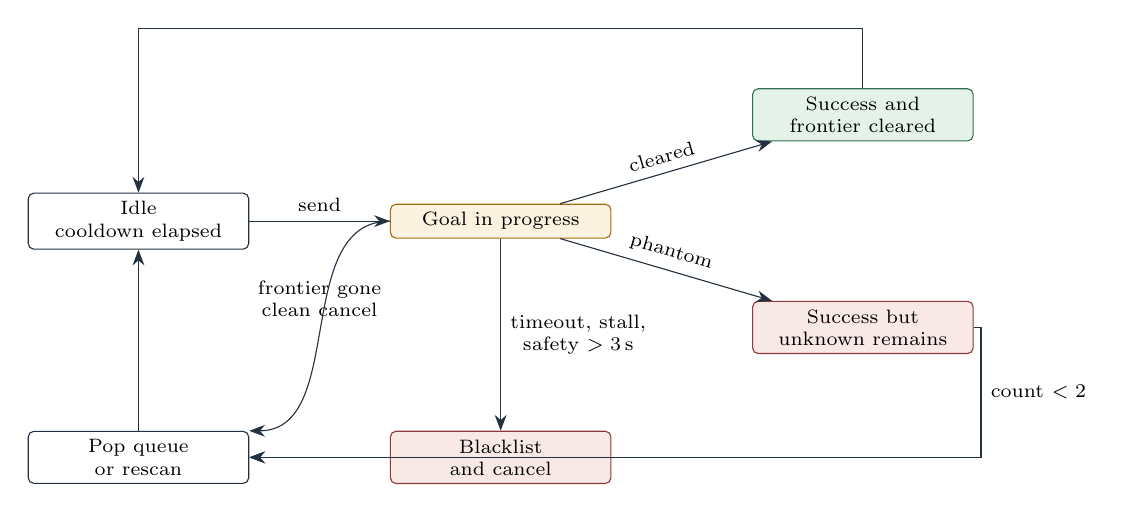
\begin{tikzpicture}[
  font=\scriptsize,
  st/.style={draw=linec, rounded corners=2pt, align=center, fill=white,
             minimum width=28mm, inner sep=3pt},
  hot/.style={st, fill=goldfaint, draw=gold},
  bad/.style={st, fill=brickfaint, draw=brick},
  good/.style={st, fill=leaffaint, draw=leaf},
  arr/.style={-{Stealth[length=2mm]}, draw=linec}
]
  \node[st] (idle) at (0,0) {Idle\\cooldown elapsed};
  \node[hot] (nav) at (4.6,0) {Goal in progress};
  \node[good] (ok) at (9.2,1.35) {Success and\\frontier cleared};
  \node[bad] (ph) at (9.2,-1.35) {Success but\\unknown remains};
  \node[bad] (bl) at (4.6,-3.0) {Blacklist\\and cancel};
  \node[st] (sw) at (0,-3.0) {Pop queue\\or rescan};
  \draw[arr] (idle) -- node[above] {send} (nav);
  \draw[arr] (nav) -- node[above, sloped] {cleared} (ok);
  \draw[arr] (nav) -- node[above, sloped] {phantom} (ph);
  \draw[arr] (ok) -- ++(0,1.1) -| (idle);
  \draw[arr] (ph) -- ++(1.5,0) |- node[pos=0.25, right] {count $<2$} (sw);
  \draw[arr] (nav) -- node[right, align=center] {timeout, stall,\\safety $>3$\,s} (bl);
  \draw[arr] (nav.west) to[out=180, in=0] node[above, align=center] {frontier gone\\clean cancel} (sw.north east);
  \draw[arr] (bl) -- (sw);
  \draw[arr] (sw) -- (idle);
\end{tikzpicture}%
}

\newcommand{\FigRecovery}{%
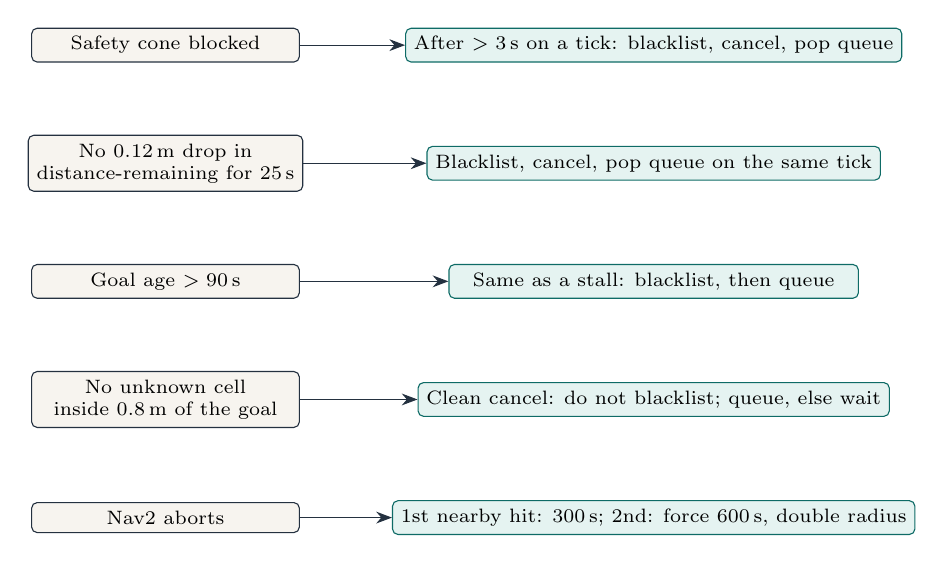
\begin{tikzpicture}[
  font=\scriptsize,
  ev/.style={draw=linec, rounded corners=2pt, align=center, fill=paper,
             minimum width=34mm, inner sep=3pt},
  act/.style={draw=teal, rounded corners=2pt, align=center, fill=tealfaint,
              minimum width=52mm, inner sep=3pt},
  arr/.style={-{Stealth[length=2mm]}, draw=linec}
]
  \node[ev] (a) at (0,0) {Safety cone blocked};
  \node[act] (a2) at (6.2,0) {After $>3$\,s on a tick: blacklist, cancel, pop queue};
  \node[ev] (b) at (0,-1.5) {No $0.12$\,m drop in\\distance-remaining for $25$\,s};
  \node[act] (b2) at (6.2,-1.5) {Blacklist, cancel, pop queue on the same tick};
  \node[ev] (c) at (0,-3.0) {Goal age $>90$\,s};
  \node[act] (c2) at (6.2,-3.0) {Same as a stall: blacklist, then queue};
  \node[ev] (d) at (0,-4.5) {No unknown cell\\inside $0.8$\,m of the goal};
  \node[act] (d2) at (6.2,-4.5) {Clean cancel: do not blacklist; queue, else wait};
  \node[ev] (e) at (0,-6.0) {Nav2 aborts};
  \node[act] (e2) at (6.2,-6.0) {1st nearby hit: $300$\,s; 2nd: force $600$\,s, double radius};
  \draw[arr] (a) -- (a2);
  \draw[arr] (b) -- (b2);
  \draw[arr] (c) -- (c2);
  \draw[arr] (d) -- (d2);
  \draw[arr] (e) -- (e2);
\end{tikzpicture}%
}

\newcommand{\FigQueue}{%
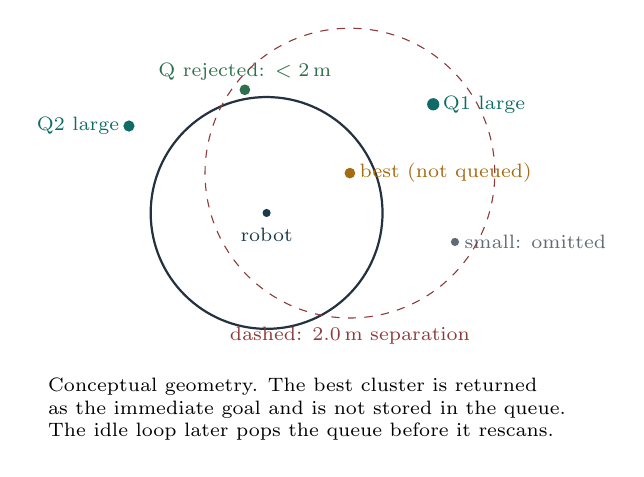
\begin{tikzpicture}[scale=0.92, font=\scriptsize]
  \draw[linec, thick] (0,0) circle (1.6);
  \fill[navy] (0,0) circle (1.6pt) node[below=2pt] {robot};
  \fill[gold] (1.15,0.55) circle (2.1pt) node[right] {best (not queued)};
  \fill[leaf] (-0.3,1.7) circle (2.1pt) node[above] {Q rejected: $<2$\,m};
  \fill[teal] (2.3,1.5) circle (2.4pt) node[right] {Q1 large};
  \fill[teal] (-1.9,1.2) circle (2.2pt) node[left] {Q2 large};
  \fill[slate] (2.6,-0.4) circle (1.6pt) node[right] {small: omitted};
  \draw[brick, dashed] (1.15,0.55) circle (2.0);
  \node[brick] at (1.15,-1.7) {dashed: $2.0$\,m separation};
  \node[align=left, anchor=north west] at (-3.15,-2.15)
    {Conceptual geometry. The best cluster is returned\\
     as the immediate goal and is not stored in the queue.\\
     The idle loop later pops the queue before it rescans.};
\end{tikzpicture}%
}

\newcommand{\FigRelax}{%
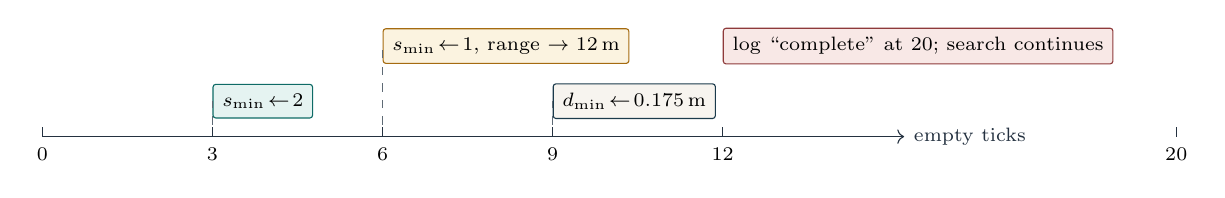
\begin{tikzpicture}[font=\scriptsize, x=0.72cm]
  \draw[->, linec] (0,0) -- (15.2,0) node[right] {empty ticks};
  \foreach \t in {0,3,6,9,12,20} {
    \draw[linec] (\t,0) -- (\t,0.12);
    \node[below] at (\t,-0.02) {\t};
  }
  \node[draw=teal, fill=tealfaint, rounded corners=1pt, anchor=west] at (3,0.45) {$s_{\min}\!\leftarrow\!2$};
  \node[draw=gold, fill=goldfaint, rounded corners=1pt, anchor=west] at (6,1.15) {$s_{\min}\!\leftarrow\!1$, range $\rightarrow 12$\,m};
  \node[draw=navy, fill=paper, rounded corners=1pt, anchor=west] at (9,0.45) {$d_{\min}\!\leftarrow\!0.175$\,m};
  \node[draw=brick, fill=brickfaint, rounded corners=1pt, anchor=west] at (12,1.15) {log ``complete'' at 20; search continues};
  \draw[slate, dashed] (3,0.15) -- (3,0.45);
  \draw[slate, dashed] (6,0.15) -- (6,1.15);
  \draw[slate, dashed] (9,0.15) -- (9,0.45);
\end{tikzpicture}%
}

\newcommand{\FigTimeline}{%
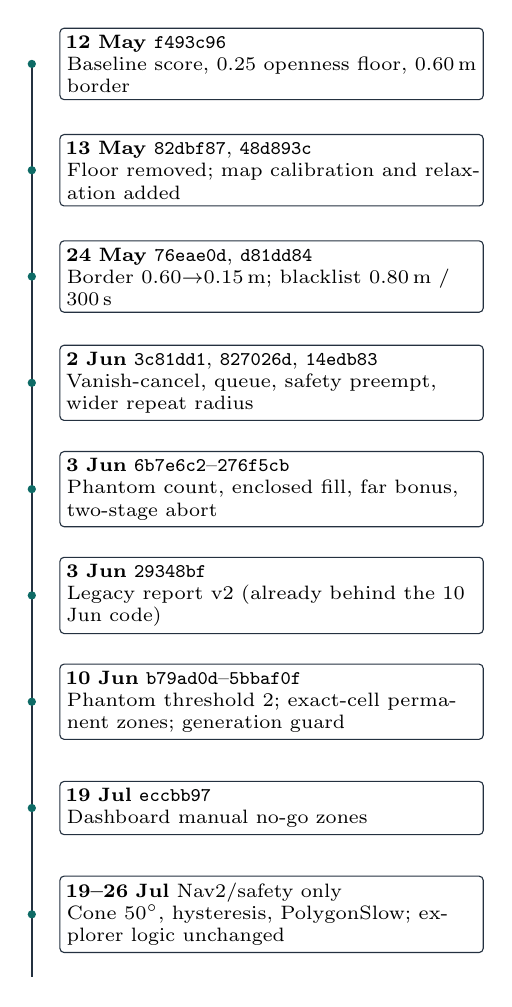
\begin{tikzpicture}[
  font=\scriptsize,
  ev/.style={draw=linec, fill=white, rounded corners=1.5pt, align=left,
             inner sep=2.5pt, text width=52mm},
  arr/.style={draw=linec, thick}
]
  \draw[arr] (0,0) -- (0,-11.6);
  \foreach \y in {0,-1.35,-2.7,-4.05,-5.4,-6.75,-8.1,-9.45,-10.8} {
    \fill[teal] (0,\y) circle (1.5pt);
  }
  \node[ev, anchor=west] at (0.35,0) {\textbf{12 May} \texttt{f493c96}\\Baseline score, 0.25 openness floor, 0.60\,m border};
  \node[ev, anchor=west] at (0.35,-1.35) {\textbf{13 May} \texttt{82dbf87}, \texttt{48d893c}\\Floor removed; map calibration and relaxation added};
  \node[ev, anchor=west] at (0.35,-2.7) {\textbf{24 May} \texttt{76eae0d}, \texttt{d81dd84}\\Border 0.60$\rightarrow$0.15\,m; blacklist 0.80\,m / 300\,s};
  \node[ev, anchor=west] at (0.35,-4.05) {\textbf{2 Jun} \texttt{3c81dd1}, \texttt{827026d}, \texttt{14edb83}\\Vanish-cancel, queue, safety preempt, wider repeat radius};
  \node[ev, anchor=west] at (0.35,-5.4) {\textbf{3 Jun} \texttt{6b7e6c2}--\texttt{276f5cb}\\Phantom count, enclosed fill, far bonus, two-stage abort};
  \node[ev, anchor=west] at (0.35,-6.75) {\textbf{3 Jun} \texttt{29348bf}\\Legacy report v2 (already behind the 10 Jun code)};
  \node[ev, anchor=west] at (0.35,-8.1) {\textbf{10 Jun} \texttt{b79ad0d}--\texttt{5bbaf0f}\\Phantom threshold 2; exact-cell permanent zones; generation guard};
  \node[ev, anchor=west] at (0.35,-9.45) {\textbf{19 Jul} \texttt{eccbb97}\\Dashboard manual no-go zones};
  \node[ev, anchor=west] at (0.35,-10.8) {\textbf{19--26 Jul} Nav2/safety only\\Cone $50^\circ$, hysteresis, PolygonSlow; explorer logic unchanged};
\end{tikzpicture}%
}

\newcommand{\FigScaleBug}{%
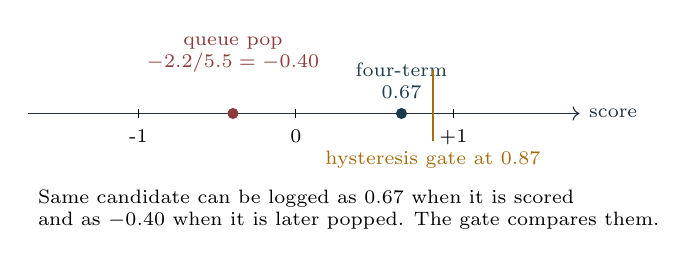
\begin{tikzpicture}[font=\scriptsize]
  \draw[->, linec] (-3.4,0) -- (3.6,0) node[right] {score};
  \foreach \x/\lab in {-2/-1, 0/0, 2/+1} {
    \draw (\x,-0.06) -- (\x,0.06);
    \node[below] at (\x,-0.08) {\lab};
  }
  \fill[navy] (1.34,0) circle (2pt) node[above=2pt, align=center] {four-term\\$0.67$};
  \fill[brick] (-0.8,0) circle (2pt) node[above=4mm, align=center, text=brick] {queue pop\\$-2.2/5.5=-0.40$};
  \draw[gold, thick] (1.74,-0.35) -- (1.74,0.55);
  \node[gold, below] at (1.74,-0.35) {hysteresis gate at $0.87$};
  \node[align=left, anchor=north west] at (-3.4,-0.85)
    {Same candidate can be logged as $0.67$ when it is scored\\
     and as $-0.40$ when it is later popped. The gate compares them.};
\end{tikzpicture}%
}

\newcommand{\FigSafetyCone}{%
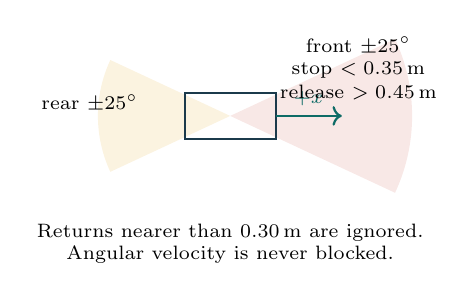
\begin{tikzpicture}[scale=1.05, font=\scriptsize]
  \fill[brickfaint] (0,0) -- (25:2.2) arc (25:-25:2.2) -- cycle;
  \fill[goldfaint] (0,0) -- (155:1.6) arc (155:205:1.6) -- cycle;
  \draw[navy, thick] (-0.55,-0.28) rectangle (0.55,0.28);
  \draw[->, teal, thick] (0.55,0) -- (1.35,0) node[midway, above] {$+x$};
  \node at (1.55,0.85) {front $\pm 25^\circ$};
  \node at (1.55,0.55) {stop $<0.35$\,m};
  \node at (1.55,0.28) {release $>0.45$\,m};
  \node at (-1.7,0.15) {rear $\pm 25^\circ$};
  \node[align=center] at (0,-1.55) {Returns nearer than $0.30$\,m are ignored.\\Angular velocity is never blocked.};
\end{tikzpicture}%
}

\newcommand{\FigExperiment}{%
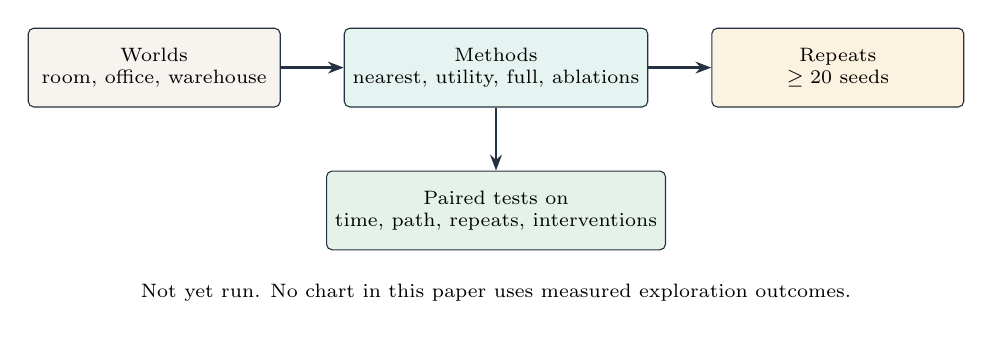
\begin{tikzpicture}[
  font=\scriptsize,
  b/.style={draw=linec, rounded corners=2pt, align=center, fill=white,
            minimum width=32mm, minimum height=10mm, inner sep=3pt},
  arr/.style={-{Stealth[length=2mm]}, draw=linec, thick}
]
  \node[b, fill=paper] (w) {Worlds\\room, office, warehouse};
  \node[b, fill=tealfaint, right=8mm of w] (m) {Methods\\nearest, utility, full, ablations};
  \node[b, fill=goldfaint, right=8mm of m] (r) {Repeats\\$\ge 20$ seeds};
  \node[b, fill=leaffaint, below=8mm of m] (y) {Paired tests on\\time, path, repeats, interventions};
  \draw[arr] (w) -- (m);
  \draw[arr] (m) -- (r);
  \draw[arr] (m) -- (y);
  \node[align=center, below=3mm of y] {Not yet run. No chart in this paper uses measured exploration outcomes.};
\end{tikzpicture}%
}

\newcommand{\FigInteraction}{%
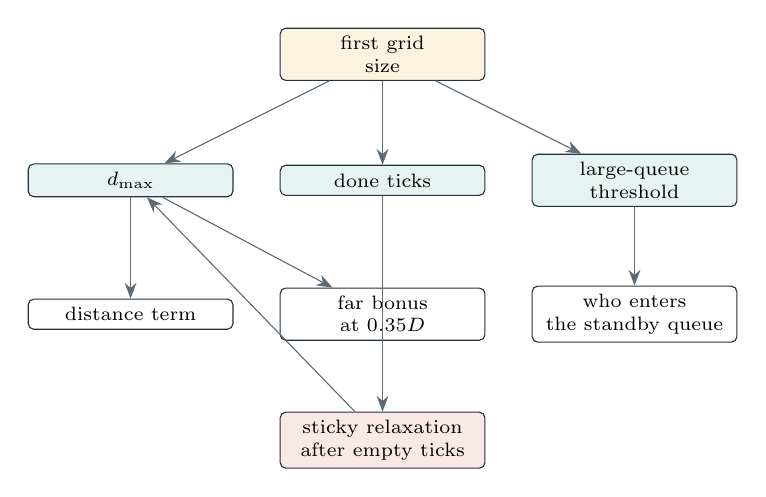
\begin{tikzpicture}[
  font=\scriptsize,
  b/.style={draw=linec, rounded corners=2pt, align=center, fill=white, inner sep=3pt,
            minimum width=26mm},
  arr/.style={-{Stealth[length=2mm]}, draw=slate}
]
  \node[b, fill=goldfaint] (map) at (0,2.2) {first grid\\size};
  \node[b, fill=tealfaint] (dmax) at (-3.2,0.6) {$d_{\max}$};
  \node[b, fill=tealfaint] (done) at (0,0.6) {done ticks};
  \node[b, fill=tealfaint] (ql) at (3.2,0.6) {large-queue\\threshold};
  \node[b] (score) at (-3.2,-1.1) {distance term};
  \node[b] (bonus) at (0,-1.1) {far bonus\\at $0.35 D$};
  \node[b] (queue) at (3.2,-1.1) {who enters\\the standby queue};
  \node[b, fill=brickfaint] (relax) at (0,-2.7) {sticky relaxation\\after empty ticks};
  \draw[arr] (map) -- (dmax);
  \draw[arr] (map) -- (done);
  \draw[arr] (map) -- (ql);
  \draw[arr] (dmax) -- (score);
  \draw[arr] (dmax) -- (bonus);
  \draw[arr] (ql) -- (queue);
  \draw[arr] (done) -- (relax);
  \draw[arr] (relax) -- (dmax);
\end{tikzpicture}%
}


\title{Failure Management for Classical Frontier\\Exploration under a Safety-Filtered Navigation Stack}
\author{Author A \and Author B\\[0.4em]
\textit{Affiliation withheld}\\
\textit{Draft for internal review, not a conference submission}}
\date{Working tree \texttt{main} at \texttt{de8209a}\\Explorer last changed in \texttt{eccbb97}}

\begin{document}
\maketitle

\begin{abstract}
This paper describes a frontier explorer that sits above an unmodified Nav2 stack and treats mapping failures as part of the decision, not only as navigation faults. The detector is the classical one: unknown occupancy cells with a free neighbour are clustered, and each cluster is scored by normalised size, Euclidean distance, heading change, and local free-space fraction. Around that score the implementation adds four mechanisms aimed at indoor maps that contain furniture voids, goals the lidar cannot clear, and stops raised by a separate laser safety filter. Enclosed unknown cells are removed by a border-seeded flood fill and then excluded by an exact cell set. A goal that Nav2 reports as reached, while unknown cells remain nearby, is counted as a phantom success and is blacklisted after two such arrivals. A standby queue of spatially separated large frontiers is popped when the safety filter, a progress stall, or a goal timeout fires. Parameters loosen on a fixed schedule if no candidate survives, but the node never latches a terminal ``done'' state. The repository records why several earlier thresholds were abandoned. It does not record a controlled comparison against nearest-frontier selection or against \texttt{explore\_lite}. The manuscript therefore states a research question and a method, and it separates that method from performance claims the present evidence cannot support.
\end{abstract}

\noindent\textbf{Keywords:} frontier exploration, occupancy grids, failure recovery, Nav2, safety filter, autonomous mapping.

\section{Introduction}
A frontier is the boundary between space a range sensor has marked free and space it has not yet observed. Sending a mobile robot to that boundary is one of the oldest practical answers to indoor exploration \cite{yamauchi1997}. The rule is easy to implement on an occupancy grid, and it remains the core of widely used ROS explorers \cite{horner2016}. It is also incomplete. A frontier behind a sofa, a frontier the planner cannot reach while a map is growing, and a frontier the robot is forbidden to approach by a hard safety stop all look, to a pure size-and-distance score, like ordinary goals.

The system studied here was built for a differential-drive robot that maps with SLAM Toolbox and navigates with Nav2. A separate node can zero forward velocity when a narrow laser cone is occupied. The exploration code was changed, over roughly ten weeks, in response to behaviours the authors recorded in commit messages: an openness cutoff that rejected every tight indoor frontier, a map-border margin that rejected every wall, repeated returns to furniture, and time spent standing still after the safety filter had already stopped the robot. Those changes are real. What the repository does not contain is a trial in which coverage, time, path length, or repeated failures were measured against a declared baseline.

The question the implementation is trying to answer is the following. On a classical frontier detector, does an explicit policy for unobservable voids, uncleared but ``reached'' goals, and safety-filter preemption reduce repeated commitment to the same map regions, without giving up frontiers that are merely narrow? This paper specifies that policy as it executes on \texttt{main}. It does not answer the question.

The contribution is therefore a precise account of an implemented policy, not a claim of superiority. In particular, the paper contributes:
\begin{enumerate}
\item a statement of the decision rule, including the enclosed-region test, the phantom-success counter, and the safety-triggered queue;
\item the distinction between that rule and stock frontier utility scoring;
\item a record of design reversals that are supported by commits, including the removal and later partial return of an openness floor;
\item an evidence audit: which statements are properties of the source, and which would require experiments that have not been run.
\end{enumerate}

\section{Related work}
Yamauchi defined a frontier as the free-space boundary of known space and selected the nearest frontier centroid \cite{yamauchi1997,yamauchi1998}. Later work replaced pure nearest-frontier choice with utility. Information-gain explorers estimate the expected new map area or the entropy reduction of a candidate viewpoint, often along a planned path \cite{makarenko2002,stachniss2005,gonzalez2002}. Comparative studies show that the ranking among nearest, greedy, and information-weighted rules depends on the environment, and that a bad cost model can erase the benefit of a better gain model \cite{holz2010}.

Detection itself has a literature. Wavefront and fast frontier detectors avoid scanning the whole grid on every cycle by growing only from newly changed free cells \cite{keidar2014,quin2014}. Sampling-based detectors, notably multiple rapidly exploring random trees, propose candidates without a full boundary extraction \cite{umari2017}. The implementation in this repository does none of those. Every selection walks the full grid.

The closest deployed relative is \texttt{explore\_lite}, whose usual citation is H\"orner's map-merging thesis \cite{horner2016}. It clusters frontiers, scores them with a weighted gain and a path cost, and can blacklist failed goals. The scorer here is in that family, with two differences that matter. Cost is Euclidean distance in the map frame, not the length of a Nav2 plan, so a frontier behind a wall can outrank a longer but open route. Gain is the cell count of the unknown cluster, not a ray-cast estimate of newly visible cells.

Nav2 and SLAM Toolbox are used as unmodified libraries \cite{macenski2020,macenski2021}. The local controller is regulated pure pursuit \cite{macenski2023}. Nothing in the explorer replaces the planner, the costmap, or the behaviour tree. No custom behaviour tree is checked into the repository, so recovery order inside Nav2 is the distribution default for the configured plugins \texttt{spin}, \texttt{backup}, and \texttt{wait}.

What is not claimed as new is frontier clustering, a linear utility, a blacklist, or flood fill of unreachable cells. Hole filling and reachable-space tests are standard mapping operations. The specific packaging that this code adds, and that a reviewer should judge only after a prior-art search, is the joint use of (i)~a permanent exact-cell exclusion of enclosed unknown space, (ii)~a counter that fires on Nav2 \emph{success} when the frontier remains, and (iii)~preemption from an external safety-stop Boolean into a geographically separated queue. Section~\ref{sec:evidence} explains why that packaging is not yet a result.

\section{Problem and scope}
\label{sec:problem}
Let the map be a grid $M$ of width $W$ and height $H$ at resolution $\rho$. Each cell is treated as free if its value is $0$ and unknown if its value is $-1$. Every other value blocks traversal in the explorer's own tests. This is stricter than a probabilistic reading: a cell at occupancy $50$ is neither a frontier seed nor free space.

The robot pose $(x,y,\psi)$ is the \texttt{map}$\rightarrow$\texttt{base\_footprint} transform. The explorer's only actuation is a \texttt{NavigateToPose} goal. It does not command velocity, and it does not read the camera or the semantic detector. Those nodes run in parallel and do not enter the score.

A frontier cluster $F$ is a connected set of unknown cells, each 8-connected to at least one free cell. The goal point $g(F)$ is not the centroid. It is the free cell, among the 8-neighbours of $F$, closest in squared index distance to the rounded mean index of $F$. The robot is therefore sent into known free space beside the boundary. The planner may still cross unknown space, because NavFn is configured with \texttt{allow\_unknown: true} and a $0.5$\,m tolerance.

The policy must choose $g$ or declare that it has no candidate, while avoiding three failure modes that the commit history names:
\begin{enumerate}
\item goals inside or on unobservable voids, such as the interior of furniture;
\item goals Nav2 can reach in the sense of its goal checker while the unknown cells remain;
\item long waits after the safety filter has already forbidden forward motion.
\end{enumerate}
The policy is not required to be optimal, to maximise information gain, or to explore a known closed world in bounded time. Termination, as implemented, is a log line rather than a stop.

\section{System context}
Figure~\ref{fig:arch} shows the nodes that affect exploration. SLAM Toolbox publishes \texttt{/map}. The explorer reads that grid, the pose, \texttt{/safety\_blocked}, and optional manual no-go zones. It sends goals to Nav2. The command path on this Jazzy configuration is controller, velocity smoother, collision monitor, then the custom safety stop, then the motor driver (Fig.~\ref{fig:chain}). Launch comments that omit the smoother and the collision monitor are stale relative to \texttt{config/nav2\_params.yaml}.

\begin{figure}[ht]
\centering
\FigArchitecture
\caption{Nodes that participate in exploration. Teal marks code in this repository. The camera and detector are omitted because they do not affect frontier scores.}
\label{fig:arch}
\end{figure}

\begin{figure}[ht]
\centering
\FigCommandChain
\caption{Velocity path implied by the Nav2 parameter file. PolygonSlow can scale a command to half speed before the safety stop independently zeros forward motion.}
\label{fig:chain}
\end{figure}

The safety stop uses a $\pm 25^\circ$ forward cone (Fig.~\ref{fig:cone}). A return between $0.30$\,m and $0.35$\,m engages the block; release requires $0.45$\,m, so the threshold does not chatter. Rear motion uses the same angular width. Yaw rate is never blocked, which is what lets Nav2 spin while translation is held. The Boolean published to the explorer is true if the forward cone is blocked or if raw wheel odometry has been silent for $0.5$\,s. A rear-only obstacle does not preempt exploration. A dead encoder does.

\begin{figure}[ht]
\centering
\FigSafetyCone
\caption{Safety geometry as launched on the hardware bringup. The shaded front sector is the only laser condition that sets \texttt{/safety\_blocked} for the explorer, together with stale wheel odometry.}
\label{fig:cone}
\end{figure}

Bringup starts SLAM at $5$\,s and Nav2 at $8$\,s. The explorer starts at $22$\,s. Its decision timer is $3$\,s, taken from \texttt{goal\_interval\_sec}. All timeouts below are checked on that timer, so a ``$3$\,s'' safety switch actually occurs on the first tick after the threshold, typically in $(3,6]$\,s.

\section{Method}
\subsection{Detection and enclosed regions}
On each full scan the grid is copied into an array. Let $U$ be the unknown cells and $C$ the free cells. Traversable cells are $C\cup U$. A 4-connected flood fill is seeded from every traversable cell on the border of the array. Unknown cells that the fill does not reach are enclosed. They are written as occupied ($100$) in the copy only. The SLAM map is not edited.

Figure~\ref{fig:enc} is a schematic of the intended case: a void with no 4-connected path to the map border never becomes a frontier. Frontiers themselves are then extracted with 8-connectivity. A diagonal gap can therefore be ``enclosed'' for the flood fill and still be a frontier adjacency. That mismatch is a property of the code, not an interpretation of it.

\begin{figure}[ht]
\centering
\FigEnclosed
\caption{Conceptual grid, not a logged map. The red cells have no 4-connected free or unknown path to the border, so they are removed before clustering. Teal cells are unknown cells that touch free space and can form a frontier.}
\label{fig:enc}
\end{figure}

Each enclosed component of at least three cells is stored twice. The centroid is kept for a marker. The cells, expanded by one cell of Chebyshev buffer, are stored as rounded world-coordinate keys $\mathrm{round}(p_x/\rho)$ and $\mathrm{round}(p_y/\rho)$. Later rejection tests are set membership, not a disk. Components whose centroids lie within $1.6$\,m of an existing permanent centroid are not entered again. The markers still draw a disk of radius $1.6$\,m, which is larger than the cell set the predicate uses.

The same rounding aliases neighbouring cells. With $\rho=0.05$\,m and an origin on a cell boundary, Python's half-to-even \texttt{round} maps cell columns $0$ and $1$ to different keys but maps columns $1$ and $2$ onto one key. The permanent mask is therefore not a perfect rendering of the buffered component.

\subsection{Pruning}
Clusters then pass the cascade in Fig.~\ref{fig:prune}. The minimum size starts at $3$ cells. The border test is an index margin $m=\max(1,\mathrm{int}(0.15/\rho))$. At the configured resolution $\rho=0.05$\,m, $0.15/0.05$ evaluates to a float slightly below $3$, and \texttt{int} truncates it to $2$. The comment in the YAML file, and the June reference note, both say three cells. The running code rejects two cells of index margin, about $0.10$\,m to the cell origin, and it can accept a goal whose centre is $0.125$\,m from the map border. The test is not a Euclidean distance to the boundary.

\begin{figure}[ht]
\centering
\FigPrune
\caption{Order of rejection inside scoring. Openness is both a hard floor and a term in the utility.}
\label{fig:prune}
\end{figure}

Distance limits are $d_{\min}=0.35$\,m and $d_{\max}=5.5$\,m on a full score. If nothing survives, the same clusters are scored again with $d_{\max}$ replaced by $\min(2\,d_{\max},\,12\,\mathrm{m})$. Openness $\Omega(g)$ is the fraction of cells in a $7\times 7$ window, radius $3$ cells, that are free. Candidates with $\Omega<0.15$ are dropped. A floor of $0.25$ was removed on 13 May 2026 because, the commit message says, it rejected all tight frontiers in warehouse and office worlds. The $0.15$ floor was reintroduced on 3 June as a narrower wedge filter. Both statements are commit messages, not measured rejection counts.

\subsection{Score}
For a surviving cluster, with $S$ the largest cluster size in the current list and $D$ the distance limit used for this pass,
\begin{align}
\sigma_{\mathrm{size}} &= |F|/S, &
\sigma_{\mathrm{dist}} &= \|g-p\|/D, \nonumber\\
\sigma_{\mathrm{head}} &= |\mathrm{wrap}(\operatorname{atan2}(g-p)-\psi)|/\pi, &
\sigma_{\mathrm{open}} &= \Omega(g).
\label{eq:terms}
\end{align}
The utility is
\begin{equation}
J(F)= 1.8\,\sigma_{\mathrm{size}} - 1.0\,\sigma_{\mathrm{dist}} - 0.5\,\sigma_{\mathrm{head}} + 0.7\,\sigma_{\mathrm{open}}.
\label{eq:score}
\end{equation}
Weights are the YAML values, which override the different defaults compiled into the node. Figure~\ref{fig:score} decomposes one hypothetical candidate. It is an arithmetic check of \eqref{eq:score}, not an observation of the robot.

\begin{figure}[ht]
\centering
\FigScore
\caption{Worked decomposition of \eqref{eq:score}. The inputs are chosen for readability. They were not taken from a log.}
\label{fig:score}
\end{figure}

If every survivor is farther than $0.35D$, the distance term is recomputed as $\max(0,\,\|g-p\|/D - \beta)$ with $\beta=\min(0.40,\,0.45\,|F|/S)$. A large far cluster sheds more of its distance penalty than a small one. The bonus does not run when any near candidate exists, even if that near candidate later loses on the other terms.

There is a second score, used only when a queued point is popped:
\begin{equation}
J_{\mathrm{pop}}= -\,\|g-p\|/D_{\mathrm{cfg}},
\label{eq:pop}
\end{equation}
where $D_{\mathrm{cfg}}$ is the current search radius, not the cap. The four-term value that ordered the queue is discarded. Figure~\ref{fig:scale} shows the consequence for the hysteresis test. While a goal is in progress the test is not consulted. On the idle path it is consulted whenever a previous goal position is still stored, and it demands $J \ge J_{\mathrm{active}}+0.20$. A popped candidate at $-0.40$ does not beat a stored four-term score of $0.67$. Whether that branch stalls a run depends on how long the previous goal position remains set; the result callback usually clears it. The scales are nonetheless not comparable, and the logged ``score'' on a queued dispatch is not \eqref{eq:score}.

\begin{figure}[ht]
\centering
\FigScaleBug
\caption{The idle hysteresis gate assumes one score definition. Queue dispatch uses another. The numerical example matches Fig.~\ref{fig:score} and \eqref{eq:pop}.}
\label{fig:scale}
\end{figure}

\subsection{Queue, preemption, and blacklist}
The highest-scoring survivor is the value returned by a full scan. It is not inserted into the queue. Up to five further survivors are inserted if they contain at least $n_L$ cells and are at least $2.0$\,m from other queued points, where $n_L$ is fixed at the first map as
\begin{equation}
n_L=\max(3 s_{\min},\,15,\,\lfloor 0.0015\,WH\rfloor).
\label{eq:nl}
\end{equation}
If no cluster meets $n_L$, the size rule is dropped and any survivor may fill the queue. Figure~\ref{fig:queue} shows the geometry. The idle loop pops this queue before it scans again, provided the queue is younger than $20$\,s. A popped point is rejected if it is blacklisted, if no unknown cell remains within $0.8$\,m, if it is closer than $d_{\min}$ or farther than the $12$\,m cap, or if it lies within $1.6$\,m of the last blacklisted point. The upper bound is the cap, not $d_{\max}$, so a queue can dispatch a goal outside the normal search radius. Because the queue is preferred whenever it is non-empty, a fast success can send a stale runner-up instead of recomputing the current best.

\begin{figure}[ht]
\centering
\FigQueue
\caption{How the standby set is built. Separation uses the blacklist radius times $2.5$, which is $2.0$\,m at the configured $0.80$\,m radius. The circle is illustrative.}
\label{fig:queue}
\end{figure}

Figure~\ref{fig:life} is the goal state machine. Figure~\ref{fig:rec} lists the transitions that cancel a goal. A vanished frontier is a clean cancel: the area is not blacklisted. A safety preemption, a stall, and a $90$\,s timeout blacklist first and then cancel. The cancel-status callback does not blacklist again. That double write was a defect fixed on 10 June (\commit{47a164d}). Stalls are defined on Nav2 feedback: the timer resets only when \texttt{distance\_remaining} falls by more than $0.12$\,m. A longer replan does not count as progress. Rotation in place can satisfy Nav2's pose progress checker, which accepts $0.3$\,rad, while the explorer still sees a stall. The two clocks are both set to $25$\,s. The YAML comment says the explorer timeout must exceed Nav2's allowance. It does not. It equals it, and the quantities differ.

\begin{figure}[ht]
\centering
\FigLifecycle
\caption{Goal lifecycle implemented by the timer and the action callbacks. ``Complete'' is not a state.}
\label{fig:life}
\end{figure}

\begin{figure}[ht]
\centering
\FigRecovery
\caption{Which events blacklist the active goal. Durations are evaluated on the $3$\,s timer, so the effective delay is the threshold plus up to one period.}
\label{fig:rec}
\end{figure}

A blacklist entry stores a timestamp, a hit count, and a timeout. Entries within $1.2$\,m are merged. The first hit uses radius $0.80$\,m and timeout $300$\,s. Later hits use radius $1.60$\,m and timeout $\min(300\cdot 2^{h-1},\,2400)$\,s. A second Nav2 abort at the same stored point additionally forces the timeout to $600$\,s and the hit counter to $10$. The radius does not grow past double; the forced counter does not enlarge it further. The first abort is deliberately not a long exclusion. The commit message states the reason: a costmap resize can abort a goal that is in fact reachable.

Phantom success is separate. On \texttt{STATUS\_SUCCEEDED}, if any unknown cell remains inside $0.8$\,m, a counter for a nearby key is incremented. At $2$, the point is blacklisted with a temporarily substituted base timeout of $600$\,s, and the hit counter is forced upward so the radius doubles. The original threshold in \commit{6b7e6c2} was $3$. The 3 June report (\commit{29348bf}) still says $3$. The threshold became $2$ on 10 June (\commit{b79ad0d}). The report is not a description of the present source.

Manual zones arrive as JSON on \texttt{/manual\_blacklist}. The dashboard converts a click from \texttt{odom} to \texttt{map}. Duration $\le 0$ does not expire. These zones are ordinary disks and are independent of the permanent cell set.

\subsection{Calibration, relaxation, and stopping}
The first occupancy grid, and only the first, may raise $d_{\max}$ to $\min(0.5 L,\,12\,\mathrm{m})$ if that value exceeds $5.5$\,m, where $L$ is the larger side of the grid in metres. It may raise the empty-tick patience to $\max(20,\,\lfloor 2L\rfloor)$. It sets $n_L$ by \eqref{eq:nl}. This uses the SLAM canvas, which includes unknown margin, and it never repeats. A first message that is smaller than the eventual map leaves the search radius at $5.5$\,m. A first message that is a large empty canvas inflates $n_L$. On a $400\times 400$ grid, $n_L=240$ cells, so the ``large frontier'' queue is often empty and the fallback admits small clusters.

If a tick finds nothing, constraints loosen and stay loose (Fig.~\ref{fig:relax}). From the configured size of $3$: tick $3$ sets the minimum size to $2$; tick $6$ sets it to $1$ and extends the search radius to $12$\,m; tick $9$ sets $d_{\min}$ to $0.175$\,m. At tick $20$ the node logs that exploration is complete. It does not set a flag, cancel the timer, or refuse later goals. The June report says the node stops sending goals. The source does not.

\begin{figure}[ht]
\centering
\FigRelax
\caption{Sticky relaxation for the configured initial size of three cells. The schedule is in ticks of the $3$\,s timer, and only ticks that find no candidate increment the counter.}
\label{fig:relax}
\end{figure}

\subsection{What the first map does to later decisions}
Figure~\ref{fig:ix} shows the only place the map size enters the policy. It does not estimate the explored area. It copies the dimensions of whichever grid arrives first into three knobs that then shape scoring, queue admission, and the meaningless completion log.

\begin{figure}[ht]
\centering
\FigInteraction
\caption{Parameter interactions that are computed, not tuned online. Relaxation can later overwrite the calibrated search radius. It does not recompute the queue threshold.}
\label{fig:ix}
\end{figure}

\section{What was tried before}
Table~\ref{tab:hist} keeps only changes that alter exploration behaviour. Hardware, teleoperation, and the cloud bridge are omitted. Motivations in the middle column are quoted from commit messages or from comments added in those commits. Where the message is silent, the cell says so.

\begin{table}[ht]
\centering
\caption{Algorithmic revisions that survive in, or explain, the current policy. Hashes are the introducing commits.}
\label{tab:hist}
\small
\begin{tabularx}{\linewidth}{@{}l l Y@{}}
\toprule
Date & Change & Stated reason \\
\midrule
12 May & Baseline utility, expansion, openness floor $0.25$, border $0.60$\,m & Restored after a branch deletion (\commit{f493c96}). \\
13 May & Openness floor removed & ``Rejecting all tight-space frontiers'' (\commit{82dbf87}). \\
13 May & One-shot calibration and relaxation & Commit title only (\commit{48d893c}). No trial log. \\
24 May & Border $0.60\rightarrow 0.15$\,m; blacklist $0.50$\,m$/90$\,s $\rightarrow 0.80$\,m$/300$\,s & YAML comment: $0.60$\,m removed every wall-adjacent frontier. \\
2 Jun & Queue, safety preemption, vanish-cancel, repeat radius & ``Zero standstill time'' is the commit's goal, not a measurement (\commit{827026d}). \\
3 Jun & Phantom counter, enclosed fill, far bonus, two-stage abort & Messages name occlusions, furniture voids, and costmap-resize aborts. \\
10 Jun & Threshold $3\rightarrow 2$; exact-cell permanent zones; callback generation & Replaces a $1.6$\,m permanent disk (\commit{5bbaf0f}). \\
19 Jul & Manual no-go & Dashboard zones (\commit{eccbb97}). \\
\bottomrule
\end{tabularx}
\end{table}

A home-return behaviour exists on branch \texttt{home\_updated} and is not on \texttt{main}. After six empty ticks that branch sends the robot to the pose captured at start. No commit on \texttt{main} explains the omission. It should not be described as part of the method.

\section{Evidence audit}
\label{sec:evidence}
No rosbag, CSV, coverage trace, or repeat-trial table is in the repository. Commit messages in July 2026 say that particular navigation faults were checked on the robot: a transform tolerance of $1.0$\,s after map-to-odometry lag near $0.6$\,s, a narrower safety cone after sideways obstacles froze the robot, and a halt when wheel odometry stopped. Those notes are not exploration experiments. They do not report sample size, a baseline, or an outcome distribution. This paper does not convert them into performance numbers.

The following statements are true because they are source behaviour, and only for that reason.
\begin{itemize}
\item The detector is a full-grid classical frontier extractor with a linear utility.
\item Enclosed unknown cells are excluded from detection for the rest of the process, and their cells are an exact blacklist.
\item Nav2 success with residual unknown is counted, and the second count blacklists.
\item The safety Boolean can preempt a goal without waiting for the $25$\,s stall timer.
\item The completion log does not stop the node.
\item The June 2026 reference report disagrees with the current source on the phantom threshold, the shape of permanent zones, the safety cone, and termination.
\end{itemize}
The following statements are not supported.
\begin{itemize}
\item The policy explores faster, shorter, or more completely than nearest-frontier or \texttt{explore\_lite}.
\item The far-frontier bonus, the queue, or the phantom counter is responsible for any share of an improvement.
\item Two phantom arrivals are a better threshold than three.
\item The $0.15$ openness floor removes only unreachable goals.
\item Exploration terminates.
\end{itemize}

Figure~\ref{fig:exp} is the minimum experiment that would start to support a conference claim. It has not been executed. Worlds already named in the history, office and warehouse, are the natural simulated maps; a hardware floor plan should be added only with a logged map. Each method should share the same Nav2 and SLAM configuration. Ablations are: no enclosed fill, no phantom counter, no queue, no far bonus, and no relaxation. Outcomes are time to a coverage threshold, path length, number of goals, number of goals within $1.2$\,m of a previous failure, safety-preemption count, and planner aborts. At least twenty repeats and a paired comparison against nearest-frontier and a gain-over-cost utility are required before any ranking is stated. Until those data exist, charts of exploration performance would be fiction, and this paper does not contain them.

\begin{figure}[ht]
\centering
\FigExperiment
\caption{Evaluation design. The figure is a protocol, not a result.}
\label{fig:exp}
\end{figure}

\section{Threats to validity and limitations}
Even after those trials, several structural choices limit what a positive result would mean.
\begin{enumerate}
\item Euclidean cost ignores walls. A win over nearest-frontier might disappear once both methods use path length, which is the cost already available from Nav2.
\item Cluster size is not visibility. A long frontier seen at a grazing angle scores like a frontier that would reveal a room.
\item The $3$\,s timer quantises every preemption. A safety stop just after a tick waits almost another full period.
\item One-shot calibration on the SLAM canvas couples a middleware detail to the decision thresholds.
\item Permanent cell keys alias under \texttt{round}, and the RViz disk overstates the exclusion.
\item The pop-score in \eqref{eq:pop} makes hysteresis and logs inconsistent with \eqref{eq:score}.
\item A dead wheel encoder is reported on the same Boolean as a forward obstacle, so a driver fault blacklists a goal that may have been feasible.
\item Semantic perception is unused. The method cannot prefer a doorway it has seen, and it also cannot be credited with semantic exploration.
\end{enumerate}

Computational cost is unprofiled. Each full scan is a linear pass over $WH$ for masks and flood fills, plus an 8-connected clustering of the frontier cells and a $7\times 7$ window per survivor. At the $3$\,s idle period this is unlikely to dominate a Raspberry Pi that is already scan-matching, but that sentence is a complexity observation, not a timing measurement. During a goal, a scan is repeated only when the queue is older than $20$\,s.

\section{Conclusion}
The repository contains a classical frontier explorer wrapped in a failure policy: drop enclosed unknown space by an exact cell set, treat an uncleared success as different from a planner abort, and leave a safety stop by a spatially separated standby goal. The policy is specific enough to reimplement from this paper together with the parameter table in the companion technical report. It is not specific enough, and not tested enough, to support a claim at IROS, ICRA, or RA-L that the robot explores better.

The defensible next paper is short. Fix the score so that a queued goal and a freshly scored goal are the same function. Latch termination or delete the claim. Log the counters the audit asks for. Run the protocol in Fig.~\ref{fig:exp} against nearest-frontier and a path-cost utility, with the enclosed-region test and the phantom counter ablated. If those two mechanisms move repeated failures and do not move coverage the wrong way, there is a result. If they do not, the honest finding is that the engineering did not change the outcome, which is also publishable and which the present documents cannot yet show.

A public Apache-2.0 repository already discloses the method. Questions of patentability are treated in the separate assessment. They should be answered by counsel before a conference version of this text is posted, and they should not be answered by treating the implementation as novel because it is local.

\begin{thebibliography}{99}
\bibitem{yamauchi1997} B.~Yamauchi, ``A frontier-based approach for autonomous exploration,'' in \emph{Proc.\ IEEE Int.\ Symp.\ Computational Intelligence in Robotics and Automation}, 1997, pp.~146--151.
\bibitem{yamauchi1998} B.~Yamauchi, ``Frontier-based exploration using multiple robots,'' in \emph{Proc.\ Int.\ Conf.\ Autonomous Agents}, 1998, pp.~47--53.
\bibitem{gonzalez2002} H.~H.~Gonz\'alez-Ba\~nos and J.-C.~Latombe, ``Navigation strategies for exploring indoor environments,'' \emph{Int.\ J.\ Robotics Research}, vol.~21, no.~10--11, pp.~829--848, 2002.
\bibitem{makarenko2002} A.~A.~Makarenko, S.~B.~Williams, F.~Bourgault, and H.~F.~Durrant-Whyte, ``An experiment in integrated exploration,'' in \emph{Proc.\ IEEE/RSJ IROS}, 2002.
\bibitem{stachniss2005} C.~Stachniss, G.~Grisetti, and W.~Burgard, ``Information gain-based exploration using Rao-Blackwellized particle filters,'' in \emph{Proc.\ Robotics: Science and Systems}, 2005.
\bibitem{holz2010} D.~Holz, N.~Basilico, F.~Amigoni, and S.~Behnke, ``Evaluating the efficiency of frontier-based exploration strategies,'' in \emph{Proc.\ ISR/ROBOTIK}, 2010.
\bibitem{keidar2014} M.~Keidar and G.~A.~Kaminka, ``Efficient frontier detection for robot exploration,'' \emph{Int.\ J.\ Robotics Research}, vol.~33, no.~2, pp.~215--236, 2014.
\bibitem{quin2014} P.~Quin, A.~Alempijevic, G.~Paul, and D.~Liu, ``Expanding wavefront frontier detection: an approach for efficiently detecting frontier cells,'' in \emph{Proc.\ Australasian Conf.\ Robotics and Automation}, 2014.
\bibitem{umari2017} H.~Umari and S.~Mukhopadhyay, ``Autonomous robotic exploration based on multiple rapidly-exploring randomized trees,'' in \emph{Proc.\ IEEE/RSJ IROS}, 2017.
\bibitem{horner2016} J.~H\"orner, ``Map-merging for multi-robot system,'' Bachelor's thesis, Charles University, Prague, 2016. Implementation basis of \texttt{explore\_lite}.
\bibitem{macenski2020} S.~Macenski, F.~Mart\'in, R.~White, and J.~Gin\'es Clavero, ``The Marathon 2: A navigation system,'' in \emph{Proc.\ IEEE/RSJ IROS}, 2020.
\bibitem{macenski2021} S.~Macenski and I.~Jambrecic, ``SLAM Toolbox: SLAM for the dynamic world,'' \emph{J.\ Open Source Software}, vol.~6, no.~61, art.~2783, 2021.
\bibitem{macenski2023} S.~Macenski, S.~Singh, F.~Mart\'in, and J.~Gin\'es, ``Regulated pure pursuit for robot path tracking,'' \emph{Autonomous Robots}, vol.~47, pp.~685--694, 2023.
\end{thebibliography}

\end{document}
